\subsection*{Task 1.5 : Cluster Validity Measure}
For our cluster validity measure, we will explain and intepret WSS (Within cluster sum of squares) and BSS (Between cluster sum of squares)
\subsubsection*{Prerequisite 1 : Sum of Square Estimate of Errors(SSE)}
Before our attempt of explaining WSS and BSS, it is essential to explain SSE (Sum of Square estimate of Errors). SSE is an evaluation metric with a plethora of applications in statistics and predictive analytics\cite{???}. It is used to evaluate a model's performance against a training set\cite{???}. The logic behind SSE is rather simple in nature. Let X an random variable and a model $y=\bar{X}$
\iffalse
\begin{center}
	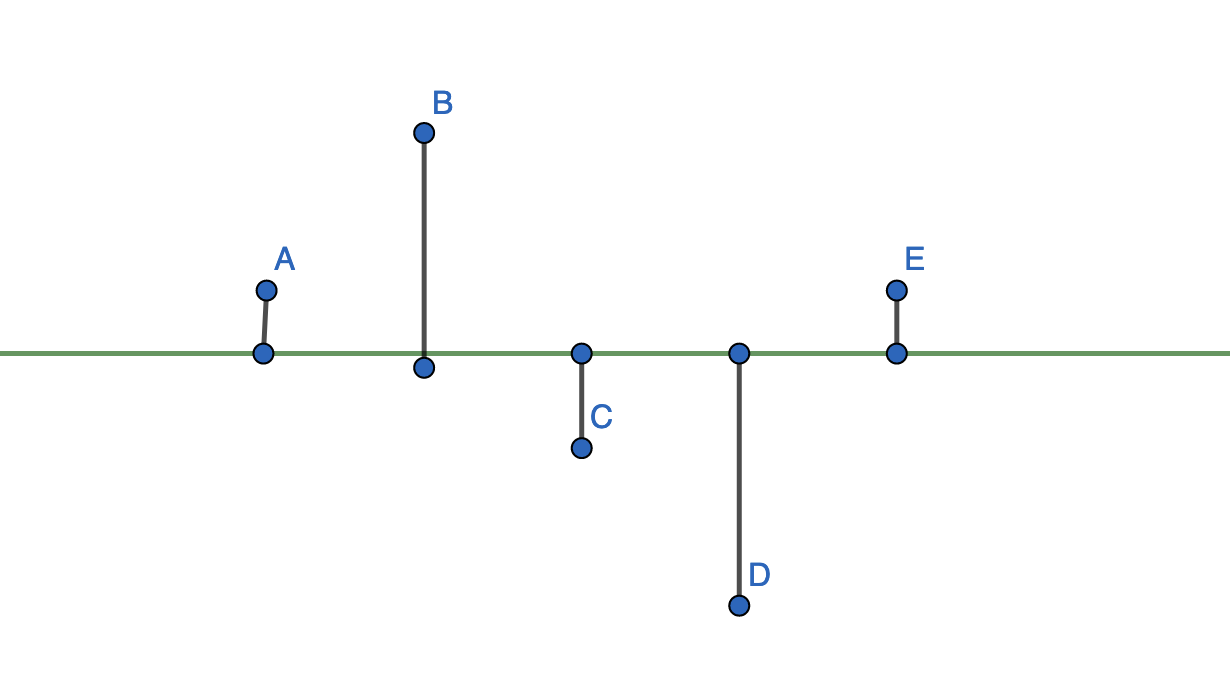
\includegraphics[scale=0.5]{res/task-1/SSE-1}				
\end{center}
\fi
We can evaluate our model's performance, by calculating the Sum of Errors, where 'error' in this case, is the distance of the observed variable from the responce of our model (i.e the mean $\bar{X}$), as follows
\iffalse
\begin{align}
	SE = \sum_{i=1}^{n}{X_i-\bar{X}}
\end{align}
\fi
Unfortunately, our evaluation metric has a fatal flaw, it allows for error's to 'cancel out' simply because they are placed beneath our model's line. It can be proven that, for the case of $y=\bar{X}$ SE is always 0.
\iffalse
\begin{align}
	SE = \sum_{i=1}^{n}{X_i-\bar{X}} \\
	SE = \sum_{i=1}^{n}{X_i} - \sum_{i=1}{n}{\bar{X}} \\
	SE = \sum_{i=1}^{n}{X_i} - n\bar{X} \\
	SE = \sum_{i=1}^{n}{X_i} - \sum_{i=1}^{n}{X_i} \\
	SE = 0 \\
\end{align}
\fi
For other models(in higher dimensions, where corellation of the involved variables is not 1), it may not be zero, but the fatal flaw remains, by cancelling errors we severely underestimate the errors involved. A more appropriate approach could be to square the distances, that would give us the Sum of Squared Errors (SSE)\\
\iffalse
\begin{align}
	SE = \sum_{i=1}^{n}{(X_i-\bar{X})}^2
\end{align}
\fi
\subsubsection*{WSS and BSS}
In the world of Clustering models performance evaluation, SSE is translated into two distinct but related ideas\cite{???}, WSS and BSS
\iffalse
\begin{figure}[H]
	\centering
	\begin{subfigure}{0.4\textwidth}
		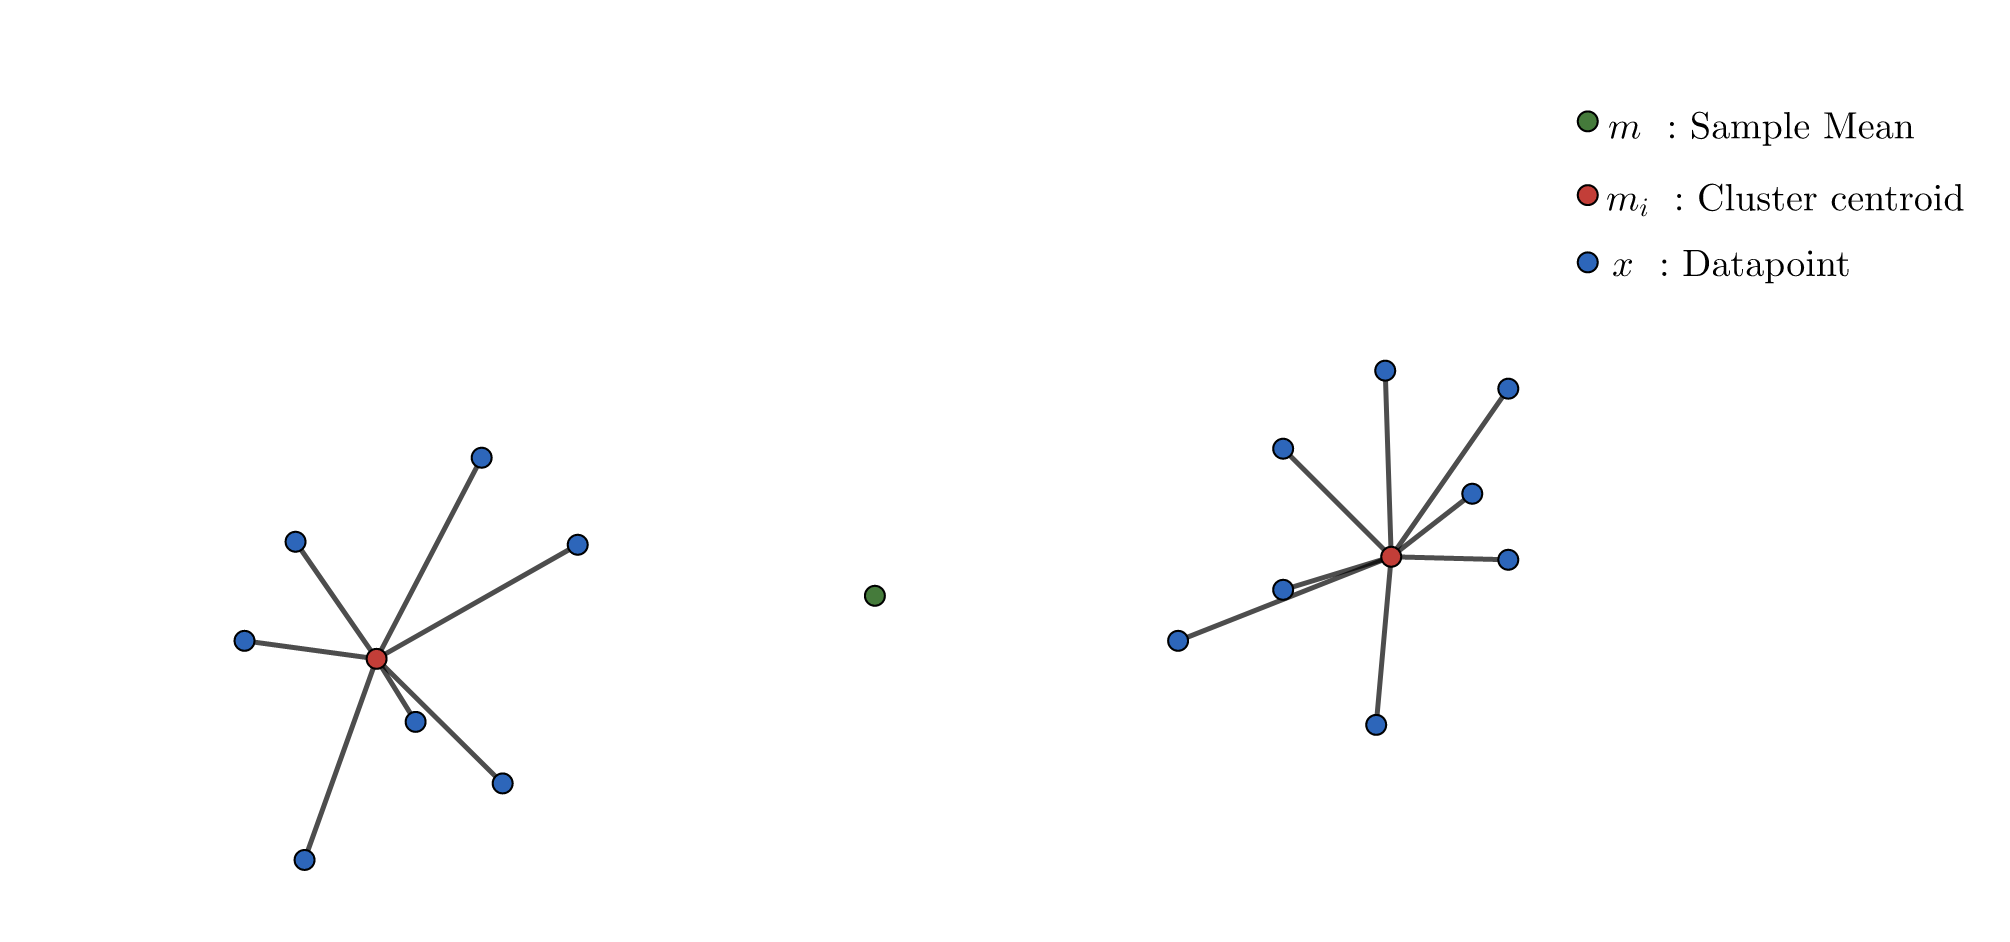
\includegraphics[width=\textwidth]{res/task-1/WSS}
		\caption{WSS}
		\label{fig:first}
	\end{subfigure}
	\hfill
	\begin{subfigure}{0.4\textwidth}
		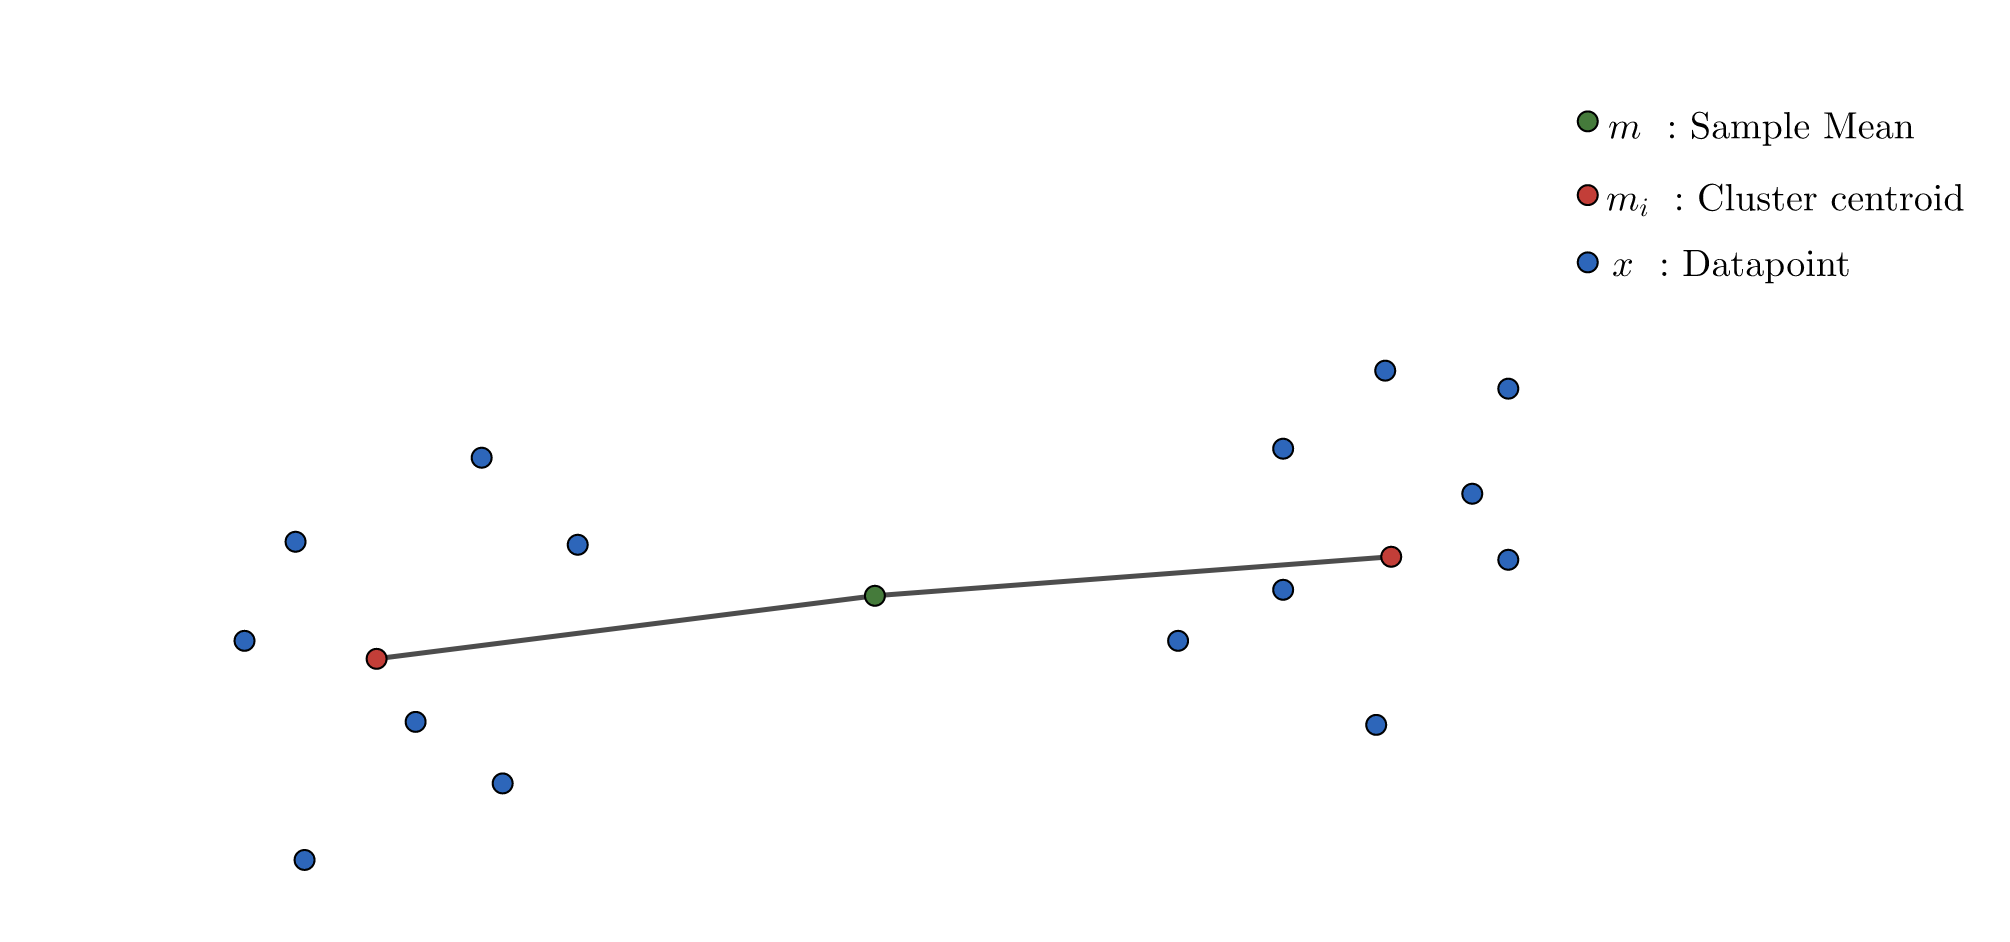
\includegraphics[width=\textwidth]{res/task-1/BSS}
		\caption{BSS}
		\label{fig:second}
	\end{subfigure}
	\hfill
	\label{fig:figures}
\end{figure}
\fi
\subsubsection*{WSS}
WSS or  Within Cluster Sum of Squares is a clustering model performance evaluation function. Our 'model' in this case is the cluster centroid and the error is the distance for each datapoint from the cluster centroid. WSS can be evaluated with the following formula\cite{???}
\iffalse
\begin{align}
	WSS = \sum_{i=1}^{k}{\sum_{x\in{C_i}}^{}{(x-m_i)^2}}	
\end{align}
\fi
Where $k$, the number of clusters involved, $C_i$ the individual cluster and $m_i$, the given cluster centroid.
\subsubsection*{BSS}
BSS or  Between Cluster Sum of Squares is a clustering model performance evaluation function, just like WSS. Our 'model' in this case is the overall data mean and the error is the distance of each cluster's centroid to the overall mean. BSS can be evaluated with the following formula\cite{???}
\iffalse
\begin{align}
	BSS = \sum_{i=1}^{k}{\abs{C_i}(m-m_i)^2}	
\end{align}
\fi
Where $k$, the number of clusters involved, $C_i$ the individual cluster and $m_i$, the given cluster centroid.
\subsubsection*{Interpretation}
A good clustering solution, would involve well separated clusters, with low WSS to BSS ratio\cite{???}. As K-Means is a heuristic based algorithm, we will not analyse WSS and BSS of a single K-Means run, but rather we will analyse their behaviour after a sequence of 100 runs. 
\iffalse
\begin{figure}[H]
	
	\centering
	\begin{subfigure}{0.4\textwidth}
		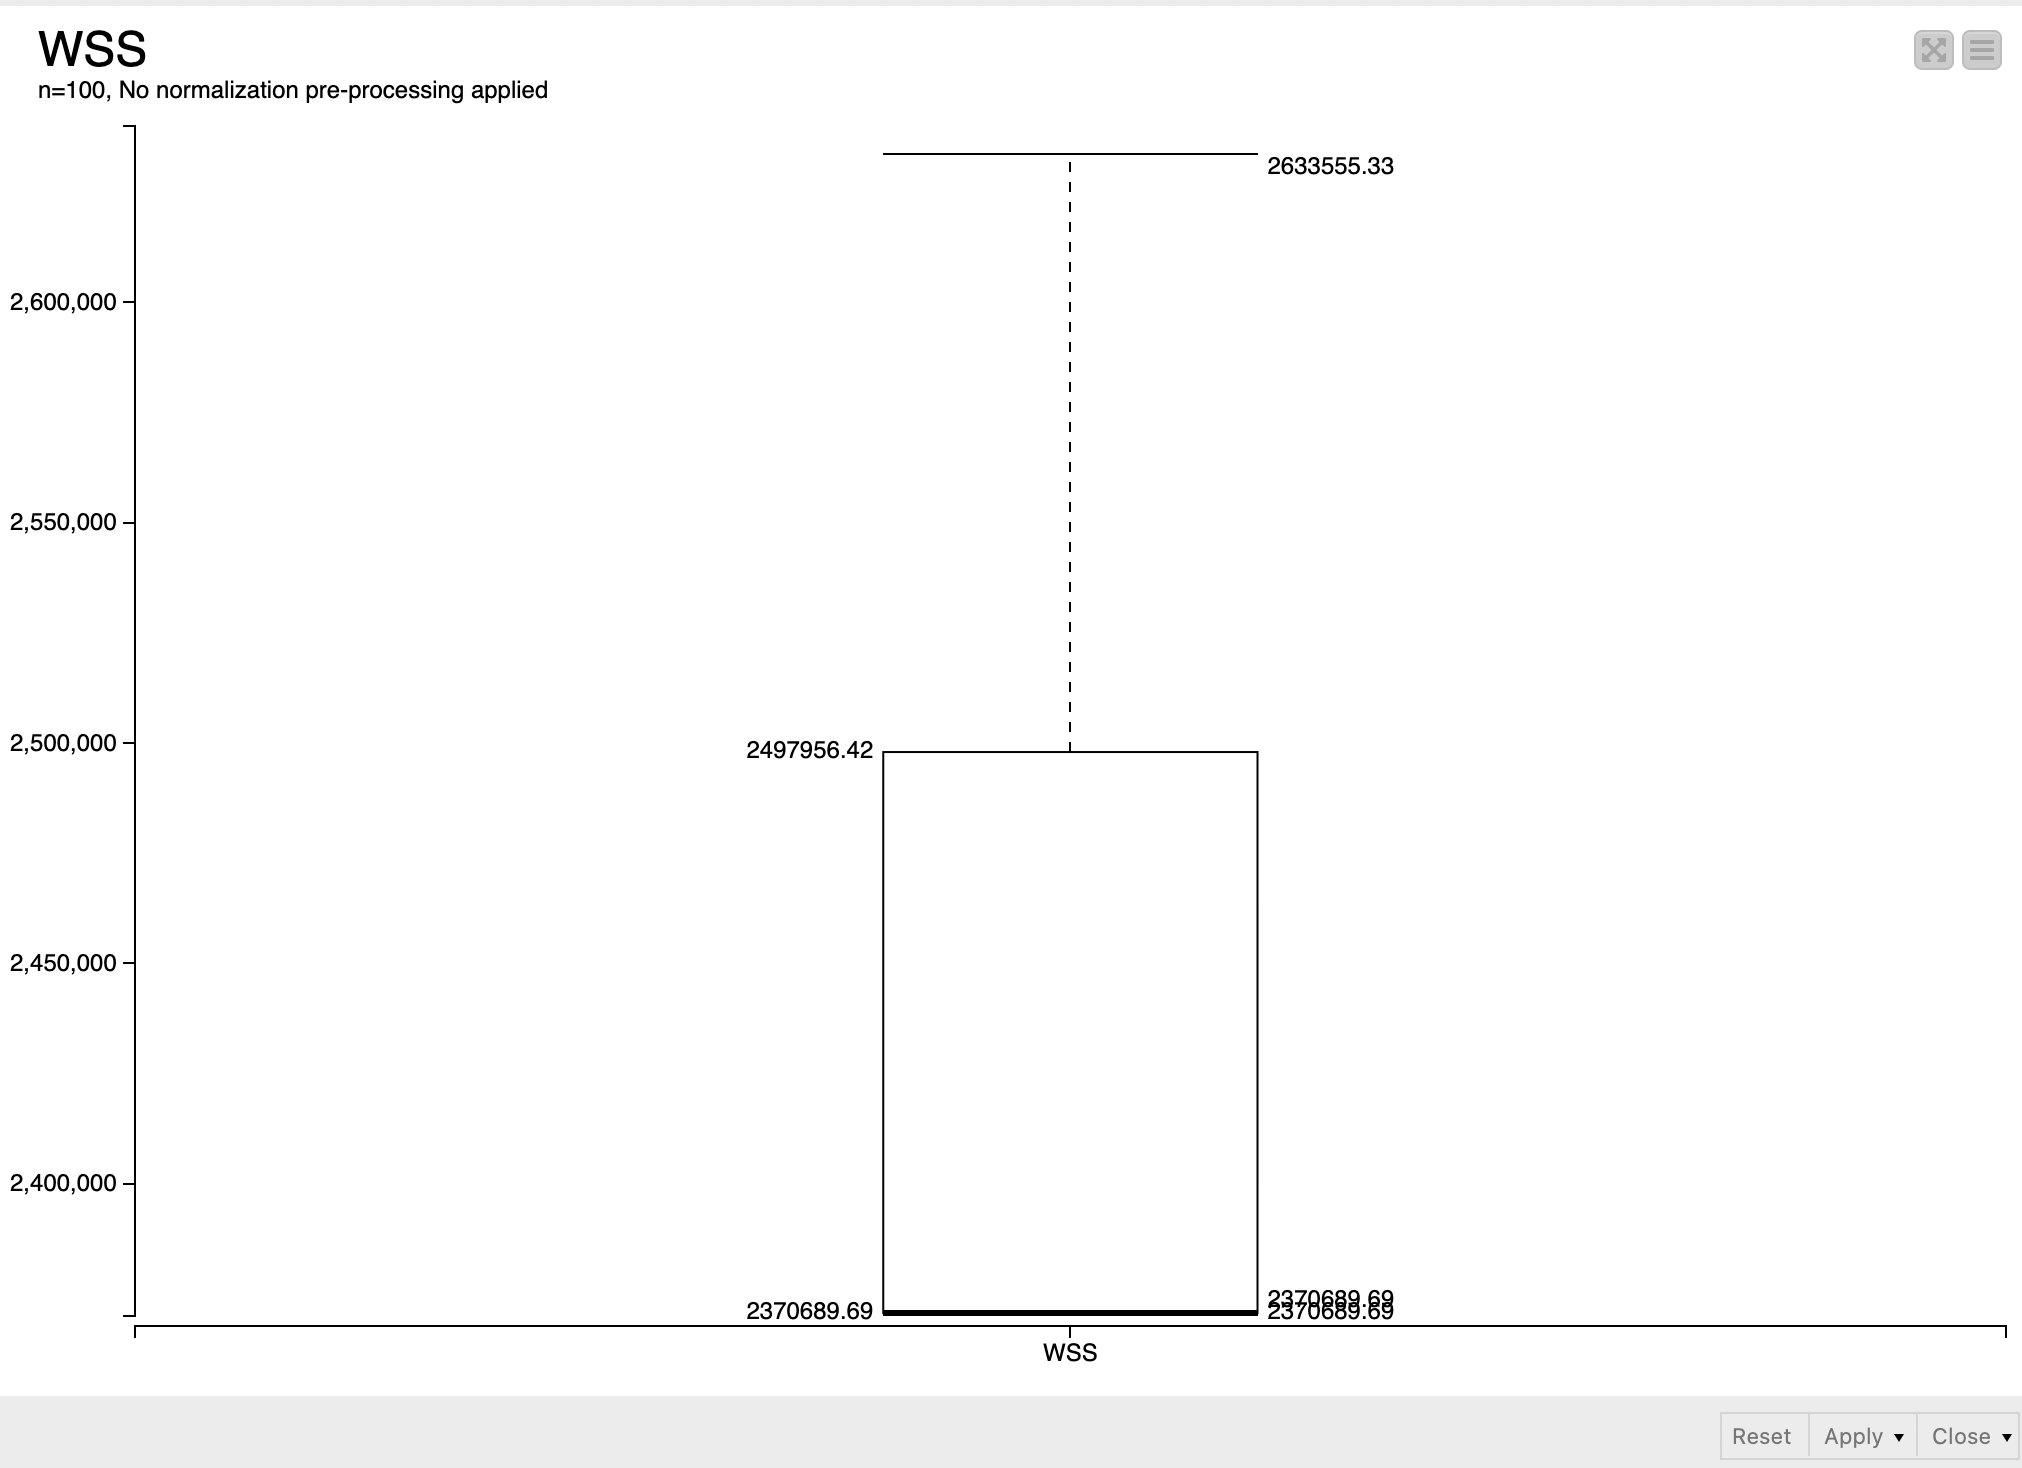
\includegraphics[width=\textwidth]{res/task-1/WSS-Knime}
		\caption{WSS}
		\label{fig:first}
	\end{subfigure}
	\hfill
	\begin{subfigure}{0.4\textwidth}
		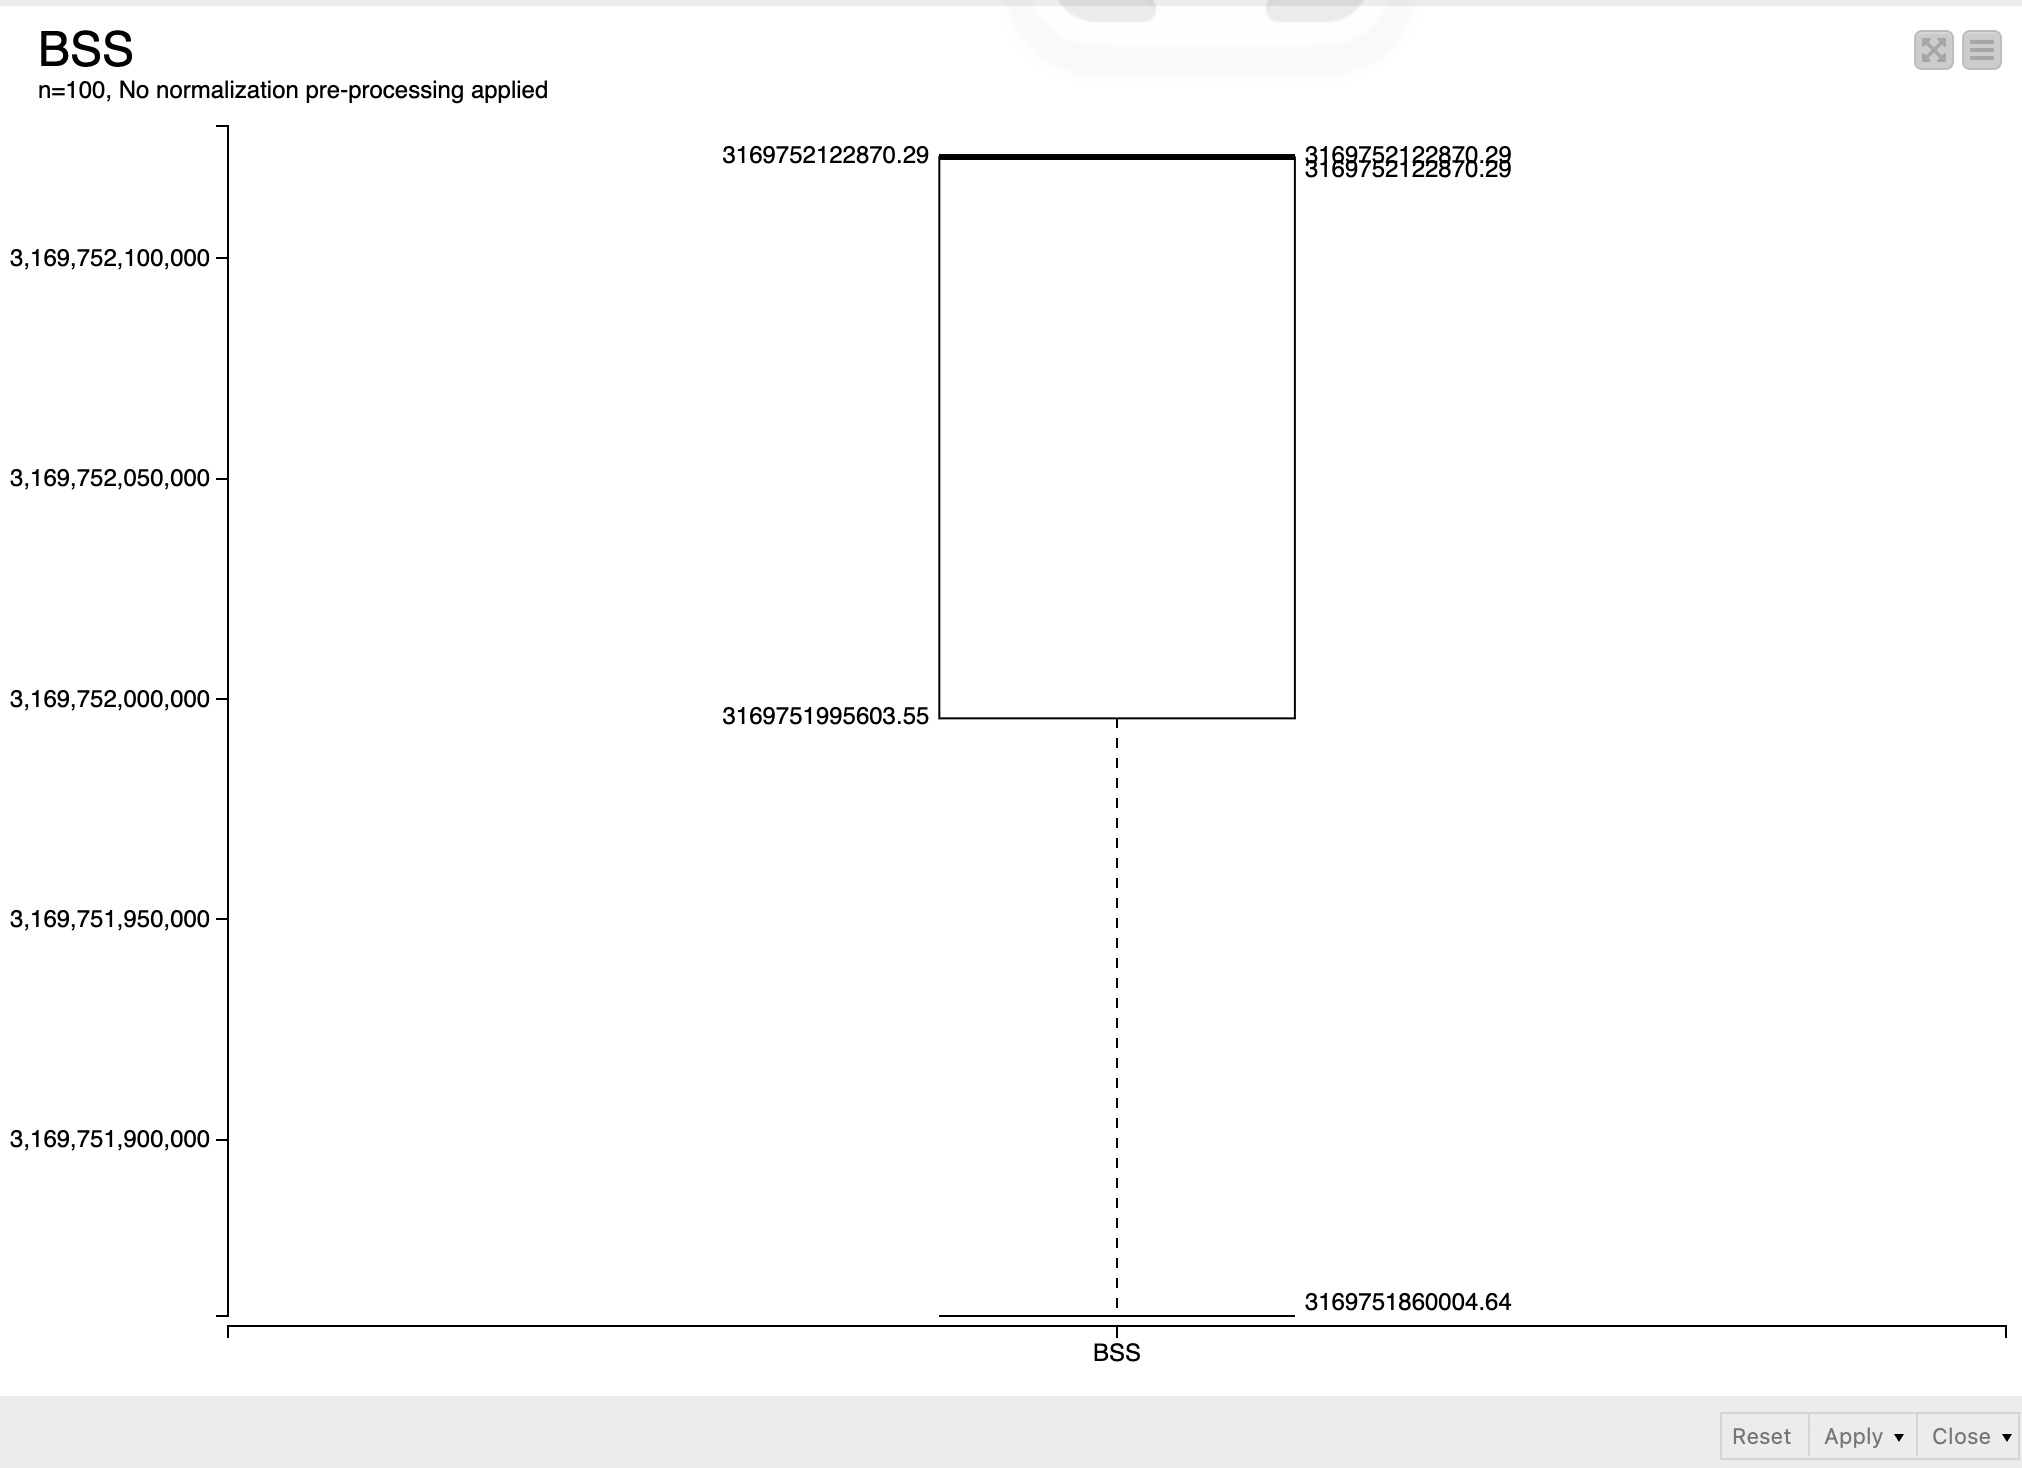
\includegraphics[width=\textwidth]{res/task-1/BSS-Knime}
		\caption{BSS}
		\label{fig:second}
	\end{subfigure}
	\hfill
	\begin{subfigure}{0.4\textwidth}
		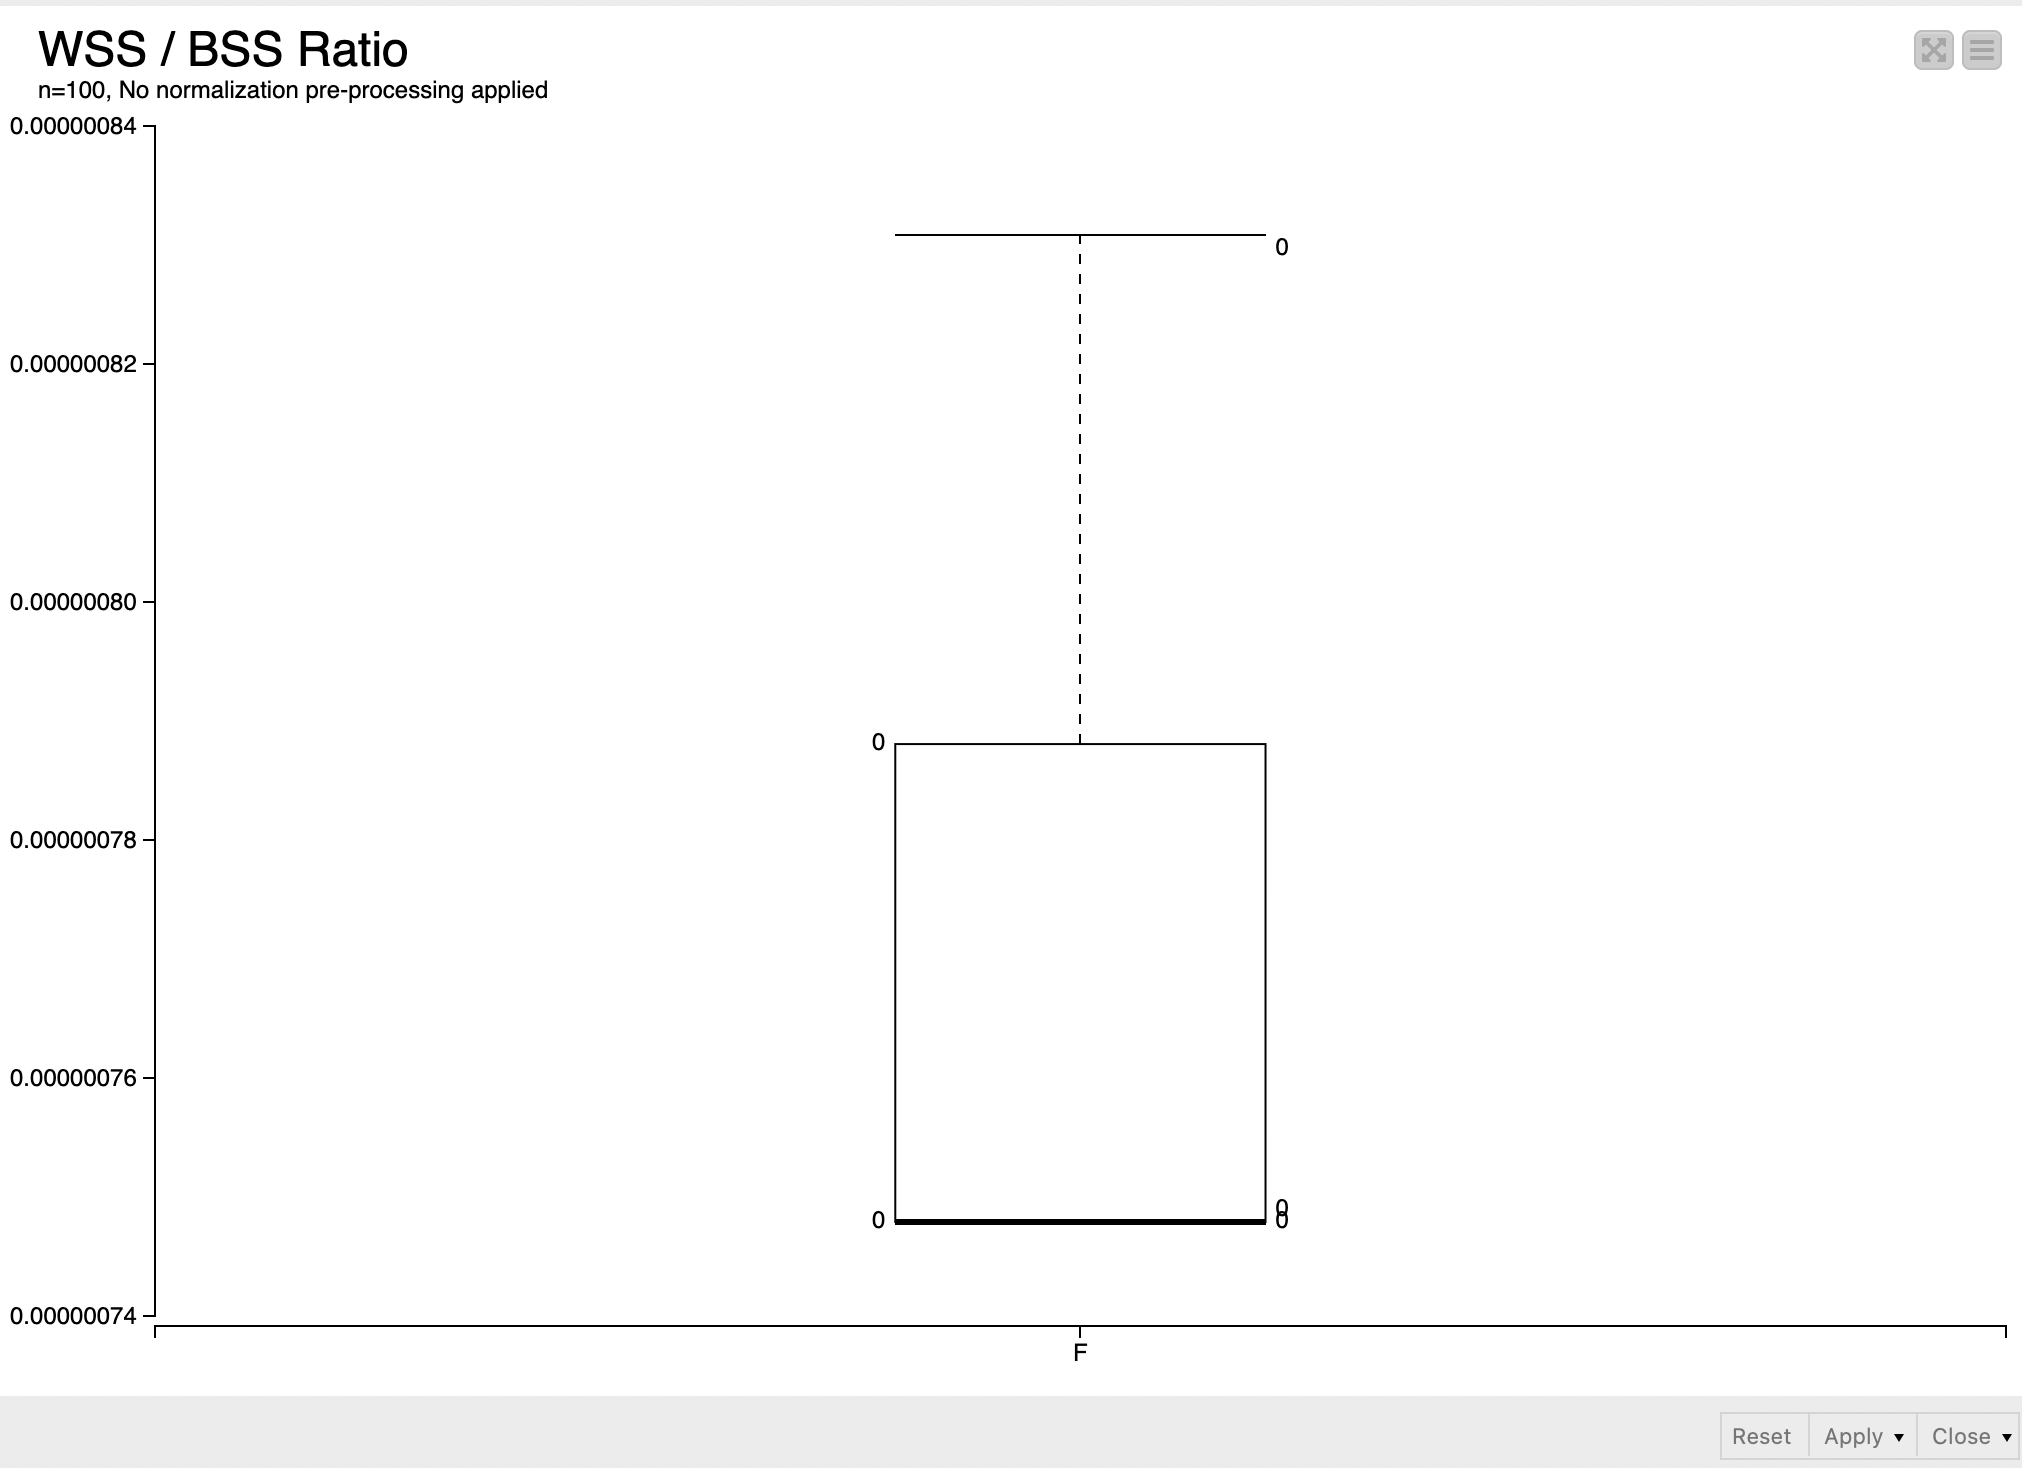
\includegraphics[width=\textwidth]{res/task-1/WSS-BSS-Ratio}
		\caption{Ratio}
		\label{fig:third}
	\end{subfigure}
	\label{fig:figures}	
\end{figure}
\fi
As we can see, The ratio of WSS to BSS is very small, something that indicates well separated clusters(i.e a good clustering solution). However, a single cluster validity measure on its own, is insufficient to provide enough evidence for a meaningful clustering. Taking into consideration our observations from Task 1.3 and Task 1.4, this clustering \cite{???}is not meaningful, is full of
errors, mainly due to the absence of the normalisation pre-processing step.
\section{Task 2}
\subsection{The effects of normalisation on plot1}
a
\subsection{The effects of normalisation on plot2}
b
\subsection{The effects of normalisation on plot3a,3b,3c}
c	
\subsection{The effects of normalisation on WSS and BSS}
d





%which leaves the algorithm vulnerable to distortion due to the different scales, measurement units and sizes of the variables in question. The following figure is part of the output of a simple 'Statistics' Node
%Without Normalization
%\begin{table}[H]
%	\begin{tabular}{llllllllllll}
%		Column&Min &Mean &	Median & Max  & Std. Dev.  \\
%		Hue&0.48&0.9574&?&1.71&0.2286 \\
%		Proline&278&746.8933&?&1,680&314.9075 \\
%		&  &  &  & 
%	\end{tabular}
%\end{table}


